% !TeX root = ../Thesis.tex

\section{Visualisierte Sichten auf das Gesamtsystem}

\subsection*{Gesammtsystem Sequenz Diagramm (Nicolas Groß)}


\begin{figure}[hbt!]
%\centering
    \begin{minipage}[t]{1\textwidth} % Breite, z.B. 1\textwidth		
        \caption{Sequenz Diagramm Gesamt System} % Überschrift
        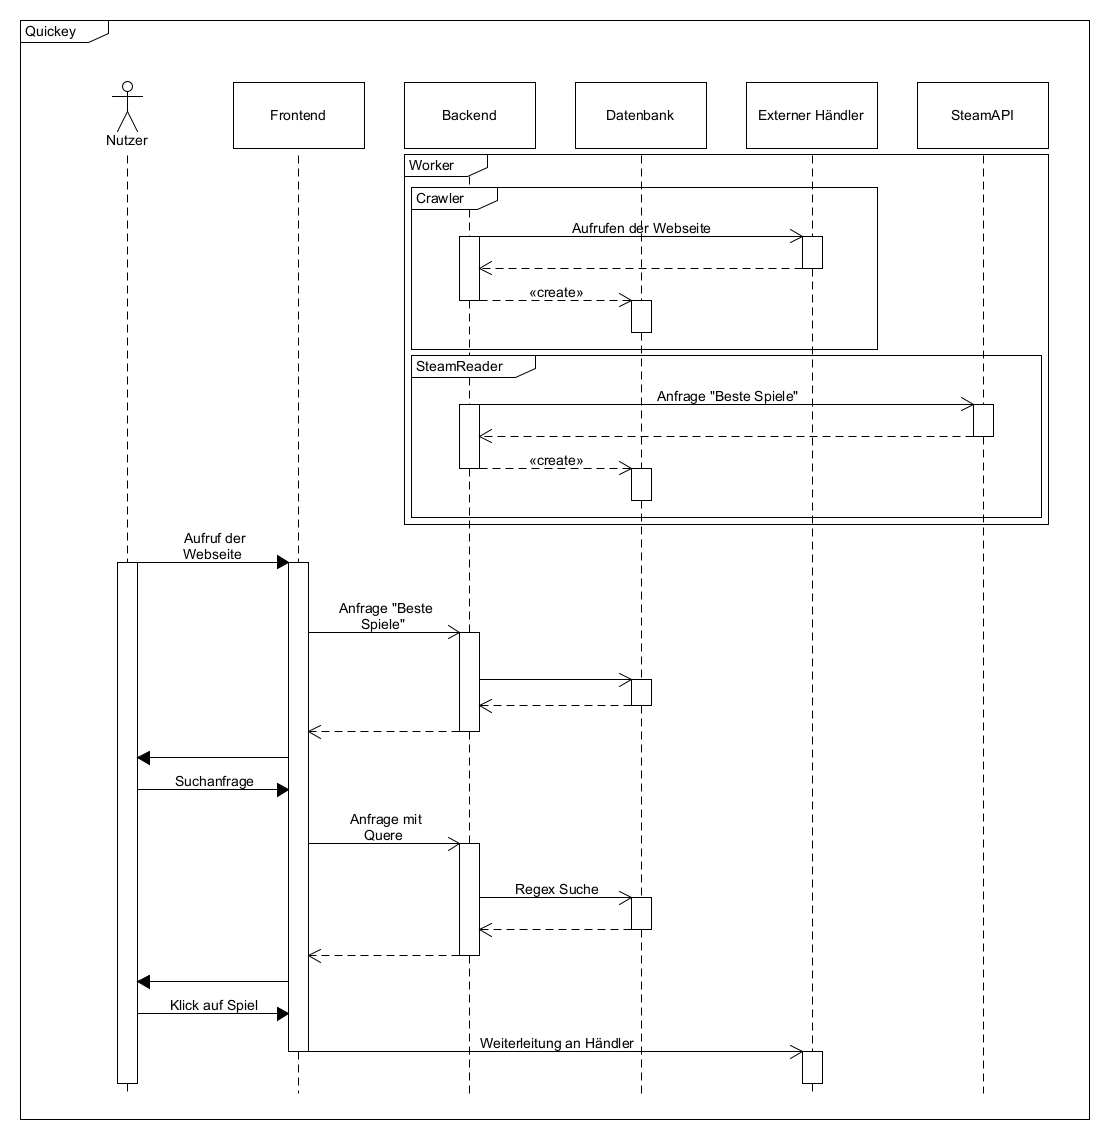
\includegraphics[width=1\textwidth]{img/sequence_system.png}\\ % Pfad
        \source{Eigene Darstellung} % Quelle
    \end{minipage}
\end{figure}
\newpage
\subsection*{Gesamtsystem Use-Case Diagramm (Niklas Hardes)}

Im Folgenden ein Use-Case Diagramm als Visualisierung zum Gesamtsystem:

\begin{figure}[hbt!]
%\centering
    \begin{minipage}[t]{.8\textwidth} % Breite, z.B. 1\textwidth		
        \caption{Use-Case Diagramm Gesamt System} % Überschrift
        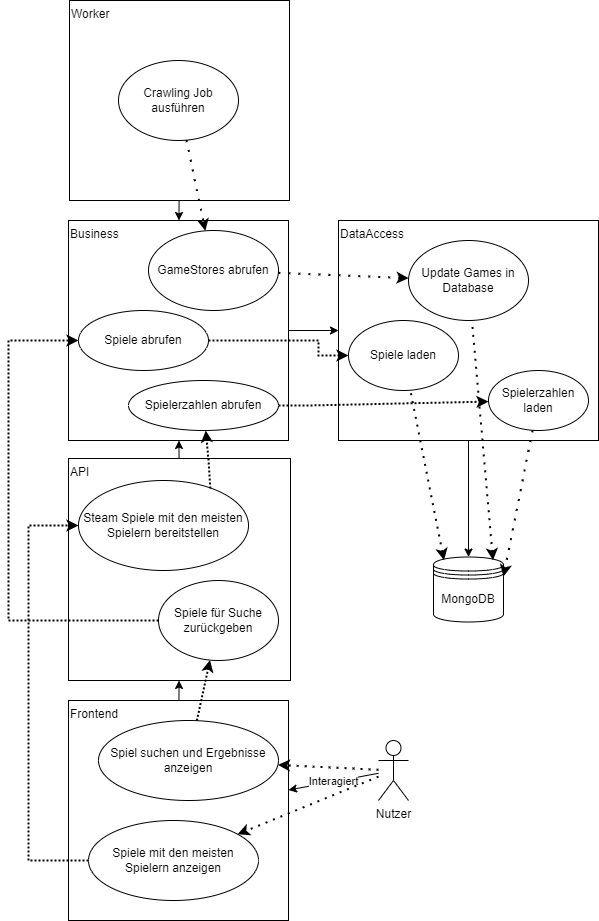
\includegraphics[width=1\textwidth]{img/use_case_gesamt_system.png}\\ % Pfad
        \source{Eigene Darstellung} % Quelle
    \end{minipage}
\end{figure}

\newpage
\subsection*{Gesamtsystem Deployment Diagramm (Robert Hesselmann)}
\begin{figure}[hbt!]
%\centering
    \begin{minipage}[t]{1\textwidth} % Breite, z.B. 1\textwidth		
        \caption{Deployment Diagramm Gesamt System} % Überschrift
        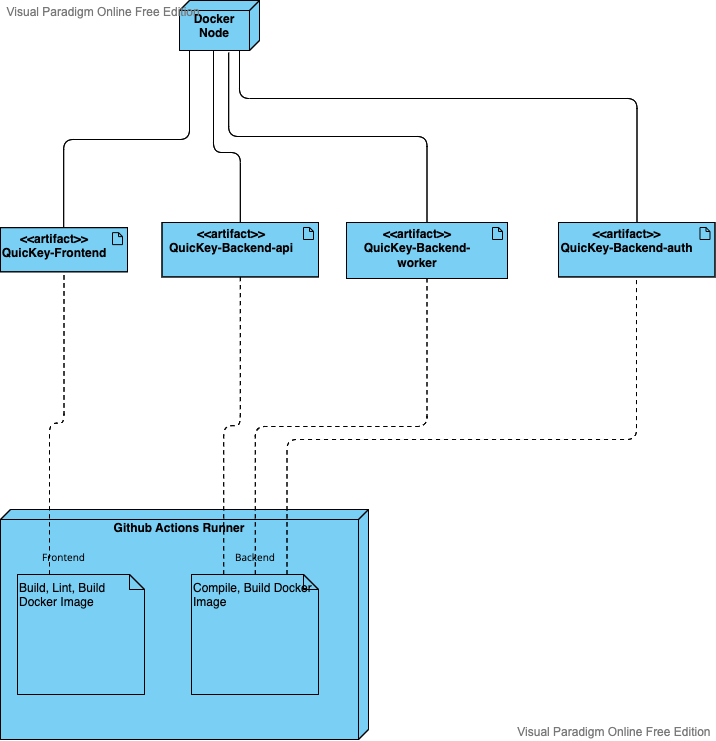
\includegraphics[width=1\textwidth]{img/deployment_system.png}\\ % Pfad
        \source{Eigene Darstellung} % Quelle
    \end{minipage}
\end{figure}
